\chapter{Model-Based Locomotion Control}
\label{sec:model_based_control}

Predicting the full floating-base dynamics over a long horizon can be expensive
for real-time control. Model-based locomotion controllers therefore use two
layers \cite{legged_optimization, cheetah_mpc}. An MPC plans the motion of the
centre of mass and the contact forces on a reduced-order model. A Whole-Body
Controller then turns this plan into joint torques, using the full dynamics and
the actuator limits.\\
\
The TITA controller has the same structure.
Section~\ref{subsec:dfcip_mpc} presents the DFCIP-based MPC, and
Section~\ref{subsec:wbc_dfcip} presents the WBC.


\section{Double Forces Constrained Inverted Pendulum MPC}
\label{subsec:dfcip_mpc}

The predictive controller used for TITA is based on the Double Forces
Constrained Inverted Pendulum (DFCIP). The model describes the centre of mass
as a point mass supported by two ground reaction forces, one for each wheel.
The motion of the wheeled support is represented by a virtual unicycle located
at the midpoint between the wheel contacts.\\
\
Figure~\ref{fig:dfcip_model} shows how the model sits on top of the real robot.
The red point is the CoM whose dynamics depend on the forces 
which came from the wheel contacts.
%
\begin{figure}[H]
    \centering
    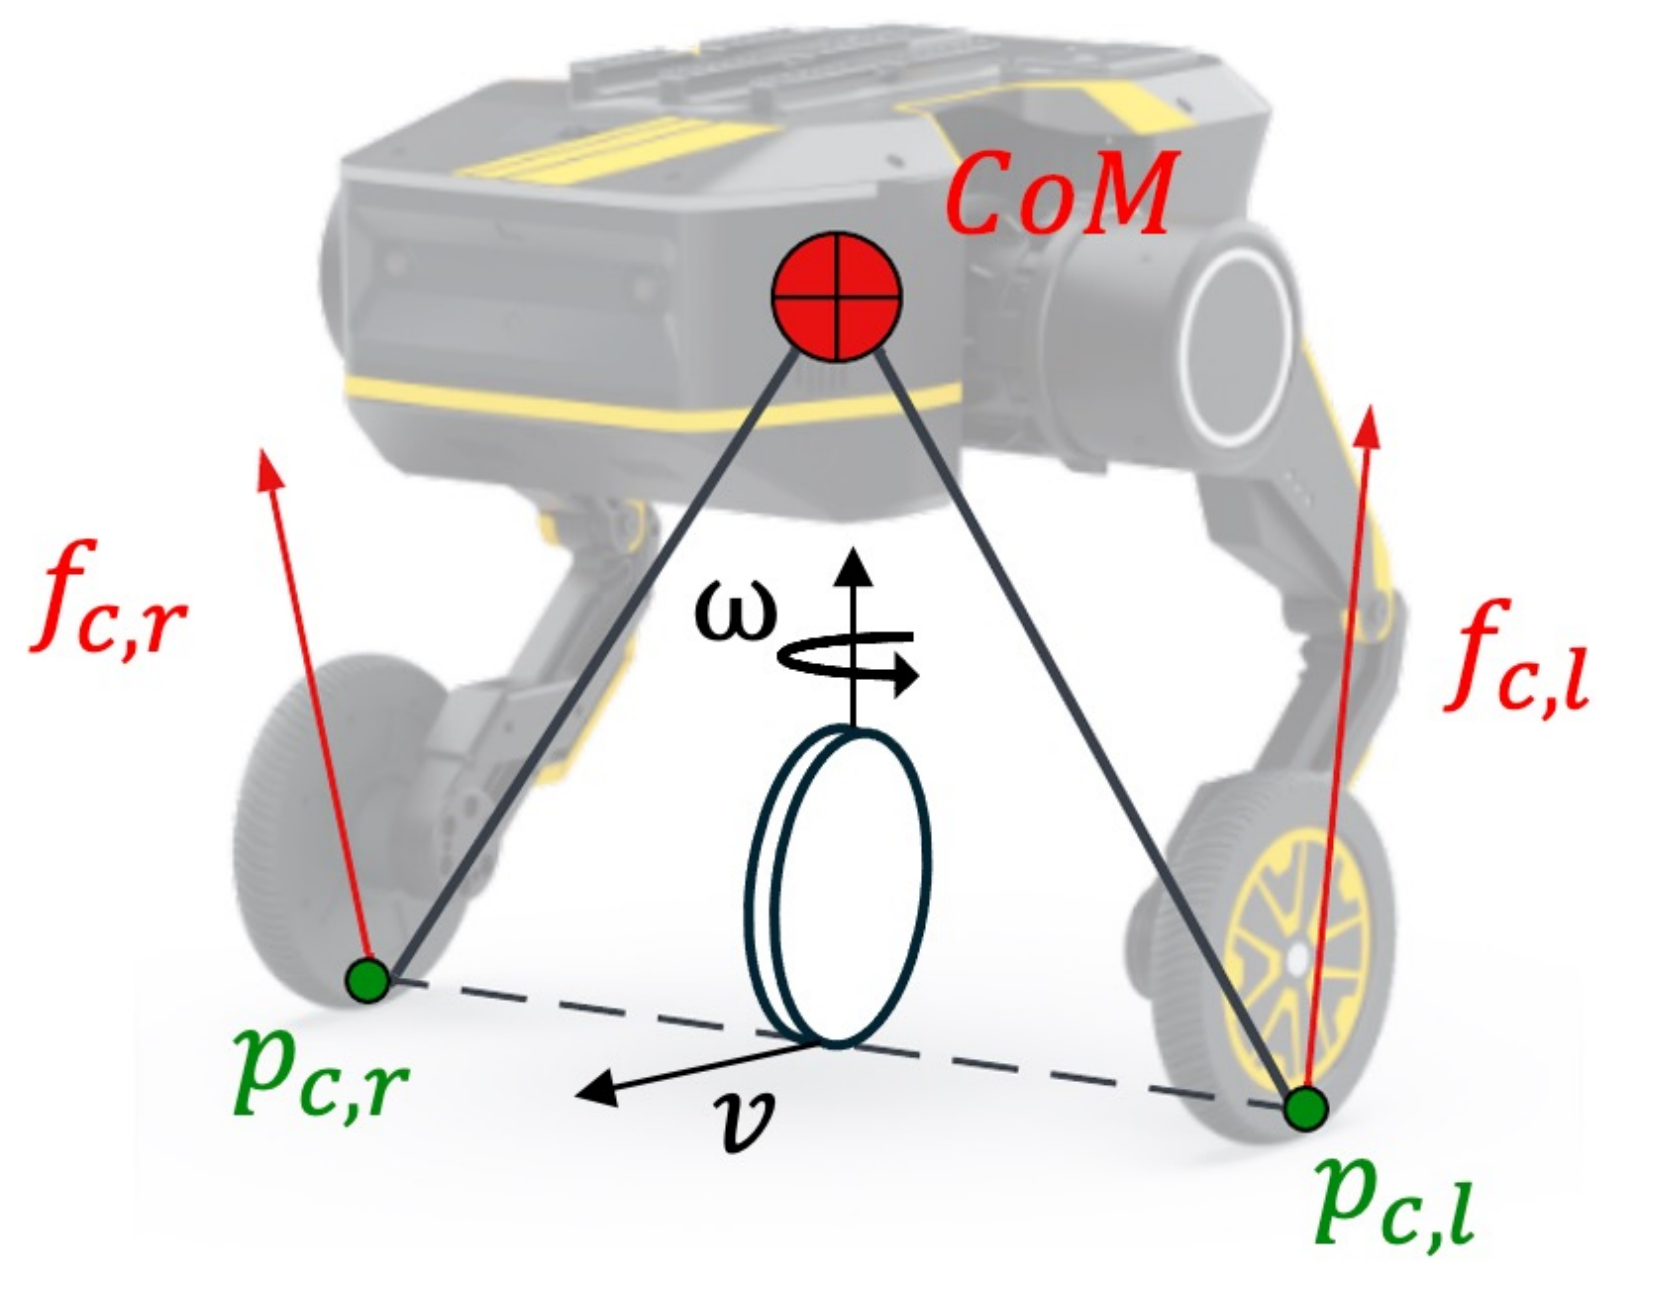
\includegraphics[width=0.6\textwidth]{images/dfcip_model.png}
    \caption{DFCIP template model overlaid on TITA. The CoM is a point mass
    supported by the contact forces \(f_{c,l}\) and \(f_{c,r}\) (denoted
    \(\mathbf{F}_L\) and \(\mathbf{F}_R\) in the text), applied at the wheel
    contacts \(p_{c,l}\) and \(p_{c,r}\). The virtual unicycle at their
    midpoint moves with forward speed \(v\) and yaw rate \(\omega\).}
    \label{fig:dfcip_model}
\end{figure}
%
\noindent The DFCIP state is
\begin{equation}
    \mathbf{x}
    =
    \begin{bmatrix}
        \mathbf{p}_{\mathrm{CoM}}^{\top} &
        \mathbf{v}_{\mathrm{CoM}}^{\top} &
        \mathbf{c}^{\top} &
        v_{c,z} &
        \theta &
        v &
        \omega
    \end{bmatrix}^{\top}
    \in\mathbb{R}^{13},
    \label{eq:dfcip_state}
\end{equation}
%
where $\mathbf{p}_{\mathrm{CoM}}$ and $\mathbf{v}_{\mathrm{CoM}}$ are the
centre-of-mass position and velocity. The vector $\mathbf{c}$ denotes the
midpoint between the two wheel contacts, while $v_{c,z}$ is its vertical
velocity. The heading angle, forward speed, and yaw rate of the virtual
unicycle are denoted by $\theta$, $v$, and $\omega$.\\
\
At each update, MPC optimizes a sequence of control inputs
$U = (\mathbf{u}_0, \ldots, \mathbf{u}_{N-1})$ over the prediction
horizon with the form
%
\begin{equation}
    \mathbf{u}
    =
    \begin{bmatrix}
        a &
        a_{c,z} &
        \alpha &
        \mathbf{F}_{L}^{\top} &
        \mathbf{F}_{R}^{\top}
    \end{bmatrix}^{\top}
    \in\mathbb{R}^{9}.
    \label{eq:dfcip_input}
\end{equation}
%
The first element, $\mathbf{u}_0$ of the optimized control sequence, is used to construct the WBC
references. The control components are the forward, angular and vertical acceleration
of the CoM, and the ground reaction forces applied to the wheel contact points.
\
The centre-of-mass dynamics are
%
\begin{equation}
    \dot{\mathbf{p}}_{\mathrm{CoM}}
    =
    \mathbf{v}_{\mathrm{CoM}},
    \qquad
    \dot{\mathbf{v}}_{\mathrm{CoM}}
    =
    \mathbf{g}
    +
    \frac{1}{m}
    \left(
        \mathbf{F}_{L}
        +
        \mathbf{F}_{R}
    \right).
    \label{eq:dfcip_com_dynamics}
\end{equation}
%
The midpoint between the wheel contacts follows the unicycle dynamics
%
\begin{equation}
\begin{aligned}
    \dot{c}_x
        &=
        v\cos\theta, &
    \dot{c}_y
        &=
        v\sin\theta, \\
    \dot{c}_z
        &=
        v_{c,z}, &
    \dot{v}_{c,z}
        &=
        0, \\
    \dot{\theta}
        &=
        \omega, &
    \dot{v}
        &=
        a, \qquad
    \dot{\omega}
        =
        \alpha.
\end{aligned}
\label{eq:dfcip_unicycle_dynamics}
\end{equation}
%
The equations for $\dot{c}_x$ and $\dot{c}_y$ enforce the nonholonomic
structure of the wheeled base: the support midpoint moves along the direction
defined by $\theta$ and has no independent lateral-velocity input. The model is
discretized using forward Euler integration with prediction time step
$dt_{\mathrm{mpc}}$.\\
\
Let $d$ denote the distance between the wheels. Their contact positions are
reconstructed from the midpoint and heading:
%
\begin{equation}
\begin{aligned}
    \mathbf{p}_{c,L}
        &=
        \mathbf{c}
        +
        \mathbf{R}_{z}(\theta)
        \begin{bmatrix}
            0 & d/2 & 0
        \end{bmatrix}^{\top}, \\
    \mathbf{p}_{c,R}
        &=
        \mathbf{c}
        -
        \mathbf{R}_{z}(\theta)
        \begin{bmatrix}
            0 & d/2 & 0
        \end{bmatrix}^{\top}.
\end{aligned}
\label{eq:dfcip_contact_positions}
\end{equation}
%
Since the DFCIP does not include an explicit rotational state for the complete
robot, a moment constraint is introduced to ensure the balance
%
\begin{equation}
    \mathbf{r}_{M,k}
    =
    \left(
        \mathbf{p}_{c,L,k}
        -
        \mathbf{p}_{\mathrm{CoM},k}
    \right)
    \times
    \mathbf{F}_{L,k}
    +
    \left(
        \mathbf{p}_{c,R,k}
        -
        \mathbf{p}_{\mathrm{CoM},k}
    \right)
    \times
    \mathbf{F}_{R,k}.
    \label{eq:dfcip_moment_residual}
\end{equation}
%
Penalizing this residual couples the location of the centre of mass to the
left--right force distribution. During turning, for example, the optimizer can
vary the tangential and vertical components of the two forces while limiting
the unmodelled resultant moment.\\
\
The DFCIP objective contains a larger set of possible tracking residuals. The stage cost is
%
\begin{equation}
\begin{aligned}
    \ell_k = 
        &w_{p_{xy}}
        \left(
            p_{\mathrm{CoM},xy,k}
            -p_{\mathrm{CoM},xy,k}^{\mathrm{ref}}
        \right)^2
        +w_{p_z}
        \left(
            p_{\mathrm{CoM},z,k}
            -p_{\mathrm{CoM},z,k}^{\mathrm{ref}}
        \right)^2
        \\
        &+w_{v_{xy}}
        \left(
            v_{\mathrm{CoM},xy,k}
            -v_{\mathrm{CoM},xy,k}^{\mathrm{ref}}
        \right)^2
        +w_{v_z}
        \left(
            v_{\mathrm{CoM},z,k}
            -v_{\mathrm{CoM},z,k}^{\mathrm{ref}}
        \right)^2
        \\
        &+w_c\left(c_k-c_k^{\mathrm{ref}}\right)^2
        +w_{v_c}
        \left(v_{c,z,k}-v_{c,z,k}^{\mathrm{ref}}\right)^2
        +w_{\theta}
        \left(\theta_k-\theta_k^{\mathrm{ref}}\right)^2
        \\
        &+w_v\left(v_k-v_k^{\mathrm{ref}}\right)^2
        +w_{\omega}\left(\omega_k-\omega_k^{\mathrm{ref}}\right)^2
        \\
        &+w_a\left(a_k-a_k^{\mathrm{ref}}\right)^2
        +w_{a_z}
        \left(a_{c,z,k}-a_{c,z,k}^{\mathrm{ref}}\right)^2
        +w_{\alpha}
        \left(\alpha_k-\alpha_k^{\mathrm{ref}}\right)^2
        \\
        &+\sum_{i\in\{L,R\}}
        \left[
            w_{F_{xy}}
            \left(F_{i,xy,k}-F_{i,xy,k}^{\mathrm{ref}}\right)^2
            +w_{F_z}
            \left(F_{i,z,k}-F_{i,z,k}^{\mathrm{ref}}\right)^2
        \right]
        \\
        &+w_{\mathrm{eq}}
        \left[
            v_{c,z,k}^{2}
            +r_{M,k}
            +\sum_{i\in\{L,R\}}
             \min\left(F_{i,z,k},0\right)^2
        \right]
\end{aligned}
\label{eq:dfcip_stage_cost}
\end{equation}
%
Where momentum is expressed as 
%
\begin{equation}
    r_{F_z,k}
    =
    \min\left(F_{L,z,k},0\right)^2
    +
    \min\left(F_{R,z,k},0\right)^2.
    \label{eq:dfcip_unilateral_force}
\end{equation}
%
It is zero when both vertical forces are nonnegative and increases when either
wheel force would pull on the ground. The residual $v_{c,z,k}^{2}$ keeps the
virtual wheel midpoint on the flat contact surface. These relations are
treated as soft constraints through the large coefficient
$w_{\mathrm{eq}}$.\\
\
The reference generator assigns
%
\begin{equation}
\begin{aligned}
    p_{\mathrm{CoM},z}^{\mathrm{ref}}
        &= z_{\mathrm{target}}, \\
    v_{\mathrm{CoM},z}^{\mathrm{ref}}
        &= 0, \\
    v_{c,z}^{\mathrm{ref}}
        &= 0, \\
    \mathbf{F}_{L}^{\mathrm{ref}}
        &=
        \begin{bmatrix}
            0 & 0 & mg/2
        \end{bmatrix}^{\top}, \\
    \mathbf{F}_{R}^{\mathrm{ref}}
        &=
        \begin{bmatrix}
            0 & 0 & mg/2
        \end{bmatrix}^{\top}.
\end{aligned}
\label{eq:dfcip_nominal_references}
\end{equation}
%
The desired forward speed and yaw rate are approached through
acceleration-limited profiles. At each prediction step,
%
\begin{equation}
\begin{aligned}
    v_{k+1}^{\mathrm{ref}}
        &=
        v_k^{\mathrm{ref}}
        +
        \operatorname{clip}
        \left(
            v^{\mathrm{cmd}}-v_k^{\mathrm{ref}},
            -a_{\max}\Delta t,
            a_{\max}\Delta t
        \right), \\
    \omega_{k+1}^{\mathrm{ref}}
        &=
        \omega_k^{\mathrm{ref}}
        +
        \operatorname{clip}
        \left(
            \omega^{\mathrm{cmd}}-\omega_k^{\mathrm{ref}},
            -\alpha_{\max}\Delta t,
            \alpha_{\max}\Delta t
        \right).
\end{aligned}
\label{eq:dfcip_velocity_ramp}
\end{equation}
%
The planar centre-of-mass velocity reference is aligned with the predicted
heading:
%
\begin{equation}
    \mathbf{v}_{\mathrm{CoM},xy,k}^{\mathrm{ref}}
    =
    v_k^{\mathrm{ref}}
    \begin{bmatrix}
        \cos\theta_k^{\mathrm{ref}} \\
        \sin\theta_k^{\mathrm{ref}}
    \end{bmatrix}.
    \label{eq:dfcip_com_velocity_reference}
\end{equation}
%
The objective therefore tracks forward speed in two related forms: through the
scalar unicycle speed $v$ and through the planar centre-of-mass velocity. The
first represents the motion of the wheel midpoint along its heading, whereas
the second regulates the global translational motion of the centre of mass.\\
\
At the terminal node, input-dependent terms are removed and an additional
stability residual is introduced:
%
\begin{equation}
    \mathbf{r}_{\mathrm{stab},N}
    =
    \mathbf{p}_{\mathrm{CoM},xy,N}
    -
    \mathbf{c}_{xy,N}.
    \label{eq:dfcip_terminal_stability}
\end{equation}
%
The terminal cost is
%
\begin{equation}
\begin{aligned}
    \ell_N =
        &w_{p_{xy}}
        \left(
            p_{\mathrm{CoM},xy,N}
            -p_{\mathrm{CoM},xy,N}^{\mathrm{ref}}
        \right)^2
        +w_{p_z}
        \left(
            p_{\mathrm{CoM},z,N}
            -p_{\mathrm{CoM},z,N}^{\mathrm{ref}}
        \right)^2
        \\
        &+w_{v_{xy}}
        \left(
            v_{\mathrm{CoM},xy,N}
            -v_{\mathrm{CoM},xy,N}^{\mathrm{ref}}
        \right)^2
        +w_{v_z}
        \left(
            v_{\mathrm{CoM},z,N}
            -v_{\mathrm{CoM},z,N}^{\mathrm{ref}}
        \right)^2
        \\
        &+w_c
        \left(
            c_N-c_N^{\mathrm{ref}}
        \right)^2
        +w_{v_c}
        \left(
            v_{c,z,N}-v_{c,z,N}^{\mathrm{ref}}
        \right)^2
        +w_{\theta}
        \left(
            \theta_N-\theta_N^{\mathrm{ref}}
        \right)^2
        \\
        &+w_v
        \left(
            v_N-v_N^{\mathrm{ref}}
        \right)^2
        +w_{\omega}
        \left(
            \omega_N-\omega_N^{\mathrm{ref}}
        \right)^2
        \\
        &+w_{\mathrm{eq}}
        \left[
            v_{c,z,N}^{2}
            +\left(
                p_{\mathrm{CoM},xy,N}-c_{xy,N}
            \right)^2
        \right]
\end{aligned}
\label{eq:dfcip_terminal_cost}
\end{equation}
%
The terminal condition encourages the centre-of-mass projection to return over
the midpoint of the two wheels. It acts as a reduced stability objective at the
end of the finite horizon. Moment balance and unilateral-force penalties are
stage terms and are not included in the implemented terminal cost.\\
\
The tasks solved directly by the TITA DFCIP-MPC are:

\begin{itemize}
    \item regulating the centre-of-mass $p_{\mathrm{CoM}}$;
    \item tracking the centre-of-mass velocity $v_{\mathrm{CoM}}$;
    \item tracking the forward speed of the wheeled support $v$;
    \item tracking the commanded yaw rate $\omega$;
    \item regularizing forward, vertical, and yaw accelerations $a$, $a_{c,z}$, $\alpha$;
    \item distributing the ground reaction forces between the two wheels $\mathbf{F}_L$, $\mathbf{F}_R$;
    \item regularizing tangential and vertical contact forces around their nominal references $F_{i,xy}$, $F_{i,z}$;
    \item enforcing moment balance through a soft residual $r_M$;
    \item maintaining zero vertical velocity of the wheel midpoint $v_{c,z}$;
    \item penalizing negative wheel normal forces $F_{i,z}<0$;
\end{itemize}
\
Planar centre-of-mass position, the position of the virtual contact midpoint,
its vertical-velocity reference, and the absolute heading angle appear in the
general objective implementation but have zero weight in the configuration
used for this work.\\
\
The controller assumes permanent contact with flat ground. It does not
switch between stance and flight dynamics, and the contact forces are not set
to zero during any part of the prediction.\\
\
The DFCIP-MPC plans the motion of a reduced model; it does not enforce the
articulated robot's equations of motion or joint-level limits. Its contact
forces are therefore a prediction, not yet a dynamically feasible motor
command. The Whole-Body Controller (WBC) receives the first MPC control and
the measured robot state, then computes joint torques while enforcing
whole-body dynamics, rolling, friction, and joint-limit constraints
(Section~\ref{subsec:wbc_dfcip}).\\
\
For TITA, the prediction horizon contains $N$ intervals of duration
$dt_{\mathrm{mpc}}$, giving a total horizon $T = N\,dt_{\mathrm{mpc}}$.
The MPC is updated at frequency $f_{\mathrm{mpc}}$, with
$n_{\mathrm{iter}}$ solver iterations per update. The previous solution is
shifted to initialize the next OCP. The same reduced-order problem is solved
independently for each simulated environment through the batched GPU
implementation provided by MPX \cite{mpx}.

\begingroup
\small
\setlength{\tabcolsep}{4pt}
\begin{longtable}{p{0.62\textwidth} p{0.28\textwidth}}
\caption{TITA DFCIP-MPC parameters and objective weights.}
\label{tab:tita_mpc_parameters}\\
\hline
\textbf{Parameter} & \textbf{Value} \\
\hline
\endfirsthead
\hline
\textbf{Parameter} & \textbf{Value} \\
\hline
\endhead
\hline
\endfoot
\hline
\endlastfoot
\multicolumn{2}{l}{\textbf{Prediction and reduced-order model}}\\
MPC update frequency, $f_{\mathrm{mpc}}$ & 100 Hz\\
Prediction timestep, $\Delta t_{\mathrm{mpc}}$ & 0.01 s\\
Horizon length, $N$ & 50 intervals\\
Prediction horizon, $T$ & 0.5 s\\
FDDP iterations per update, $n_{\mathrm{iter}}$ & 1\\
State dimension, $n_x$ & 13\\
Control dimension, $n_u$ & 9\\
Robot mass, $m$ & 27.6898 kg\\
Wheel-contact separation, $d$ & 0.567 m\\
Gravity, $g$ & 9.81 m/s$^2$\\
\multicolumn{2}{l}{\textbf{State and input cost weights}}\\
CoM planar position, $w_{p_{xy}}$ & 0\\
CoM height, $w_{p_z}$ & $2\times10^{4}$\\
CoM planar velocity, $w_{v_{xy}}$ & $3\times10^{2}$\\
CoM vertical velocity, $w_{v_z}$ & $1\times10^{1}$\\
Wheel-midpoint position, $w_c$ & 0\\
Wheel-midpoint vertical velocity, $w_{v_c}$ & 0\\
Heading, $w_\theta$ & 0\\
Forward speed, $w_v$ & $1\times10^{1}$\\
Yaw rate, $w_\omega$ & 5\\
Forward acceleration, $w_a$ & $1\times10^{-1}$\\
Vertical acceleration, $w_{a_z}$ & $1\times10^{-1}$\\
Yaw acceleration, $w_\alpha$ & $1\times10^{-3}$\\
Horizontal contact force, $w_{F_{xy}}$ & $1\times10^{-7}$\\
Vertical contact force, $w_{F_z}$ & $1\times10^{-4}$\\
Soft-constraint penalty, $w_{\mathrm{eq}}$ & $1\times10^{6}$\\
\end{longtable}
\endgroup



\newpage
\section{Whole-Body Control}
\label{subsec:wbc_dfcip}
The WBC used for TITA turns the reduced-order MPC plan into joint torques by
solving a quadratic program (QP) over the full robot model. Its decision vector
contains generalized accelerations and the three-dimensional forces at the
left and right wheel contacts,
\[
    x = \begin{bmatrix}
        \ddot{q}^{\top} & f_L^{\top} & f_R^{\top}
    \end{bmatrix}^{\top},
    \qquad \ddot{q}\in\mathbb{R}^{n_v},
\]
where $n_v=6+n_j$ counts the six floating-base velocities and the $n_j$
actuated joints ($n_j=8$ for TITA).
The QP computes generalized accelerations and wheel contact forces while
imposing the floating-base equations of motion as equality constraints. The
actuator torques are then calculated from the optimized accelerations and
contact forces using inverse dynamics.\\
The desired WBC references are constructed from the first control input
$u_0$ of the optimized MPC sequence and the current robot state:
CoM position, velocity, and acceleration; left and right wheel trajectories;
and base yaw, angular velocity, and angular acceleration. These references
form the feedforward and PD terms of the commanded task accelerations. Joint
posture is referenced to the nominal configuration, with zero reference joint
velocity and acceleration. The whole-body QP minimizes the following weighted
quadratic cost:
\begin{equation}
\begin{aligned}
H_{\mathrm{WBC}}(x) ={}&
    w_{\mathrm{com}}
    \left\|J_{\mathrm{com}}\ddot{q}
        +\dot{J}_{\mathrm{com}}\dot{q}
        -a_{\mathrm{com}}^{\mathrm{cmd}}\right\|^2
    \\
    &+w_{\mathrm{lw}}
    \left\|J_{\mathrm{lw}}\ddot{q}
        +\dot{J}_{\mathrm{lw}}\dot{q}
        -a_{\mathrm{lw}}^{\mathrm{cmd}}\right\|^2
    +w_{\mathrm{rw}}
    \left\|J_{\mathrm{rw}}\ddot{q}
        +\dot{J}_{\mathrm{rw}}\dot{q}
        -a_{\mathrm{rw}}^{\mathrm{cmd}}\right\|^2
    \\
    &+w_{\mathrm{base}}
    \left\|J_{\mathrm{base}}^{\omega}\ddot{q}
        +\dot{J}_{\mathrm{base}}^{\omega}\dot{q}
        -\alpha_{\mathrm{base}}^{\mathrm{cmd}}\right\|^2
    \\
    &+w_{\mathrm{posture}}
    \left\|S\left(\ddot{q}
    -a_{\mathrm{posture}}^{\mathrm{cmd}}\right)\right\|^2
    +w_{\ddot{q}}\|\ddot{q}\|^2
    +\epsilon_f
        \left(\|f_L\|^2+\|f_R\|^2\right).
\end{aligned}
\label{eq:tita_wbc_cost}
\end{equation}
Here, each commanded task acceleration contains feedforward acceleration and
PD feedback. The matrix $S\in\mathbb{R}^{n_v\times n_v}$ is a diagonal
selection matrix. The complete set of objectives and hard conditions handled by the
TITA whole-body QP is:
\begin{itemize}
    \item tracking CoM translational acceleration and wheels-centre translational acceleration, 
    \item tracking base angular acceleration, 
    \item regulating hip-abduction joint acceleration toward posture $q_0$,
    \item regularizing generalized acceleration $\ddot{q}$;
    \item regularizing contact forces $f_L$ and $f_R$;
    \item enforcing floating-base Newton--Euler dynamics;
    \item enforcing rolling kinematics at the left and right wheels;
    \item constraining predicted joint velocities;
    \item constraining predicted joint positions to their limits;
    \item bounding wheel contact forces by friction pyramids;
    \item enforcing positive normal force at both wheels.
\end{itemize}
In compact form, the constrained QP is
\[
    \begin{aligned}
        \min_x\quad & H_{\mathrm{WBC}}(x),\\
        \text{subject to}\quad & A_{\mathrm{eq}}x=b_{\mathrm{eq}},\\
        & d_{\min}\le Cx\le d_{\max}.
    \end{aligned}
\]
Here, $A_{\mathrm{eq}}$ is the coefficient matrix for the equality constraints
and $b_{\mathrm{eq}}$ is their right-hand-side vector. In the implementation,
these are the variables named \texttt{A\_eq} and \texttt{b\_eq}: they stack
three rolling-constraint equations for each wheel and six floating-base
dynamics equations. Thus, the QP has twelve scalar equality
constraints. The matrix $C$ and bounds $d_{\min},d_{\max}$ collect the
inequality constraints.\\
The joint inequalities constrain the predicted state one WBC sample ahead.
For each actuated joint $j$, the QP uses
\[
\begin{aligned}
    \dot{q}_{j}^{+}
        &= \dot{q}_{j}+\Delta t_{\mathrm{wbc}}\ddot{q}_{j},\\
    q_{j}^{+}
        &= q_{j}+\Delta t_{\mathrm{wbc}}\dot{q}_{j}
           +\frac{\Delta t_{\mathrm{wbc}}^{2}}{2}\ddot{q}_{j},
\end{aligned}
\]
and imposes the hard bounds
\[
    -\dot{q}_{j,\max}\leq \dot{q}_{j}^{+}\leq \dot{q}_{j,\max},
    \qquad
    q_{j,\min}\leq q_{j}^{+}\leq q_{j,\max}.
\]
The position limits are read from the joint ranges in the MuJoCo model. The
implementation sets the velocity bound to $100\,\mathrm{rad/s}$ for every
actuated joint. The inequality block also applies a friction-pyramid bound to
each contact force in its local contact frame and enforces a positive lower
bound on the normal force.\\
The equality constraints encode the physics the QP cannot violate. They
require the wheels to roll without slipping and the accelerations to be
consistent with the floating-base dynamics under the chosen contact forces.
Both conditions are expressed through the wheel kinematics.\\
For each wheel $i\in\{L,R\}$, define the spatial Jacobian of its centre as
\[
    J_i=\begin{bmatrix} J_i^{p} \\ J_i^{\omega} \end{bmatrix}
    \in\mathbb{R}^{6\times n_v}.
\]
Its linear block $J_i^{p}$ is the wheel-centre Jacobian already introduced in the
cost ($J_L^{p}=J_{\mathrm{lw}}$, $J_R^{p}=J_{\mathrm{rw}}$); $J_i^{\omega}$
maps $\dot{q}$ to the angular velocity of the wheel,
$\boldsymbol{\omega}_i=J_i^{\omega}\dot{q}$, expressed in the world frame.
Splitting the columns into floating-base and actuated coordinates gives
\[
    J_i=\begin{bmatrix} J_{iu} & J_{ia} \end{bmatrix},
    \qquad
    J_{iu}\in\mathbb{R}^{6\times 6},\quad
    J_{ia}\in\mathbb{R}^{6\times n_j}.
\]
For the contact point, let $\mathbf{r}_i$ be the
vector from the centre of wheel $i$ to its contact point. It is not read from
the simulator's contacts but built geometrically from a virtual frame
$R_i^{\mathrm{v}}=[\,\mathbf{t}_i\;\mathbf{n}_i\;\mathbf{s}_i\,]$ attached to
the wheel centre: $\mathbf{n}_i$ is the wheel axis, $\mathbf{s}_i$ is the
in-plane direction closest to the world vertical, and
$\mathbf{t}_i=\mathbf{n}_i\times\mathbf{s}_i$ is the rolling direction. In
this frame the contact vector is fixed,
$\mathbf{r}_i=R_i^{\mathrm{v}}[0\;0\;-r_w]^{\top}=-r_w\mathbf{s}_i$, where
$r_w$ is the wheel radius. A flat, horizontal ground is therefore assumed. A contact force $f_i$, expressed in
the world frame, acts at that point; seen from the wheel centre, it becomes a
force plus the moment it generates. The matrix $T_i\in\mathbb{R}^{6\times 3}$
is defined as:
\[
    T_i=\begin{bmatrix} I_3 \\ [\mathbf{r}_i]_{\times} \end{bmatrix},
    \qquad
    T_i f_i
    =
    \begin{bmatrix}
        f_i \\
        \mathbf{r}_i \times f_i
    \end{bmatrix},
\]
where $[\mathbf{r}_i]_{\times}$ is the skew-symmetric matrix such that
$[\mathbf{r}_i]_{\times}f_i=\mathbf{r}_i\times f_i$.\\
The QP imposes the rolling constraint of the wheels at the acceleration
level, with the equation of Kameduła~\cite{kamedula_centauro}:
\[
    \left(J_i^{p}-[\mathbf{r}_i]_{\times}J_i^{\omega}\right)\ddot{q}
    =
    -\left(\dot{J}_i^{p}-[\mathbf{r}_i]_{\times}\dot{J}_i^{\omega}\right)\dot{q}
    -\boldsymbol{\omega}_i\times\left(\boldsymbol{\omega}_i^{\mathrm{v}}\times\mathbf{r}_i\right).
\]
All vectors are expressed in the world frame. Here
$\boldsymbol{\omega}_i^{\mathrm{v}}$ is the angular velocity of the virtual
frame $R_i^{\mathrm{v}}$. The frame follows the wheel when it tilts or steers
but not when it spins, so its angular velocity is the wheel one without the
component along the axis,
\[
    \boldsymbol{\omega}_i^{\mathrm{v}}
    =\left(I_3-\mathbf{n}_i\mathbf{n}_i^{\top}\right)\boldsymbol{\omega}_i .
\]
Regarding the dynamics of the system, the mass matrix $M$ and the bias vector $c$, which gathers Coriolis, centrifugal, and
gravity terms, are split by rows into an unactuated part (subscript $u$, the
first six rows) and an actuated part (subscript $a$). The unactuated rows give
\[
    M_u\ddot{q}+c_u = J_{Lu}^{\top}T_Lf_L+J_{Ru}^{\top}T_Rf_R .
\]
Once $\ddot{q}$ and $f_L,f_R$ have been found, the remaining $n_j$ actuated
rows give the torque command,
\[
    \tau = M_a\ddot{q}+c_a-J_{La}^{\top}T_Lf_L-J_{Ra}^{\top}T_Rf_R.
\]
The Jacobian-transpose products $J_{La}^{\top}T_Lf_L$ and
$J_{Ra}^{\top}T_Rf_R$ map the contact wrenches to generalized forces on the
actuated coordinates. The resulting torques form the actuator-level command
that realizes the motion selected by the whole-body optimization.

\begingroup
\small
\setlength{\tabcolsep}{4pt}
\begingroup
\begin{longtable}{p{0.62\textwidth} p{0.28\textwidth}}
\caption{TITA whole-body controller parameters and QP constraints.}
\label{tab:tita_wbc_parameters}\\
\hline
\textbf{Parameter} & \textbf{Value} \\
\hline
\endfirsthead
\hline
\textbf{Parameter} & \textbf{Value} \\
\hline
\endhead
\hline
\endfoot
\hline
\endlastfoot
\multicolumn{2}{l}{\textbf{Timing and references}}\\
WBC update frequency, $f_{\mathrm{wbc}}$ & 100 Hz\\
WBC sample time, $\Delta t_{\mathrm{wbc}}$ & 0.01 s\\
Reference lookahead, $\Delta t_{\mathrm{lookahead}}$ & 0.0 s\\
Wheel radius, $r_w$ & 0.0925 m\\
\multicolumn{2}{l}{\textbf{PD gains}}\\
CoM/base motion gains & $K_{p,\mathrm{motion}}=50$, $K_{d,\mathrm{motion}}=30$\\
Wheel gains & $K_{p,\mathrm{wheel}}=50$, $K_{d,\mathrm{wheel}}=30$\\
Joint-posture regulation gains & $K_{p,\mathrm{reg}}=100$, $K_{d,\mathrm{reg}}=20$\\
Posture-regulated joints, $\mathcal{J}_{\mathrm{posture}}$ & $\{0,4\}$ (left and right hip-abduction joints)\\
\multicolumn{2}{l}{\textbf{QP objective weights}}\\
CoM acceleration, $w_{\mathrm{com}}$ & 1.0\\
Left-wheel acceleration, $w_{\mathrm{lw}}$ & 1.0\\
Right-wheel acceleration, $w_{\mathrm{rw}}$ & 1.0\\
Base angular acceleration, $w_{\mathrm{base}}$ & 1.0\\
Posture task, $w_{\mathrm{posture}}$ & 0.1\\
Generalized-acceleration regularization, $w_{\ddot{q}}$ & $1\times10^{-12}$\\
Contact-force regularization, $\epsilon_f$ & $1\times10^{-9}$\\
\multicolumn{2}{l}{\textbf{QP constraints and solver}}\\
Friction coefficient, $\mu$ & 0.9\\
Minimum normal contact force, $F_{z,\min}$ & 5.0 N\\
Actuated-joint velocity bound, $\dot{q}_{j,\max}$ & $\pm100$ rad/s\\
Joint-position bounds, $q_{j,\min},q_{j,\max}$ & MuJoCo model joint ranges\\
QP solver & QPAX\\
Solver tolerance, $\epsilon_{\mathrm{QP}}$ & $1\times10^{-3}$\\
\end{longtable}
\endgroup
\endgroup

